\documentclass[
  journal=large,
  manuscript=article-type,
  year=2020,
  volume=37,
]{cup-journal}

\usepackage{amsmath}
\usepackage[nopatch]{microtype}
\usepackage{booktabs}

\title{$titulo$}

\author{F. Author}
\affiliation{First Division, Organization, City, Pincode, State, Country}
\email[F. Author]{first.author@address.edu}

\author{S. Author}
\affiliation{Second Division, Organization, City, Pincode, State, Country}
% \alsoaffiliation{Joint first authors}

\author{T. Author}
\affiliation{Second Division, Organization, City, Pincode, State, Country}

\author{F.T. Author}
\affiliation{Fourth Division, Organization, City, Pincode, State, Country}

\addbibresource{example.bib}

\keywords{keyword entry 1, keyword entry 2, keyword entry 3} %% First letter not capped

\begin{document}

\begin{abstract}
$introduccion$
\end{abstract}

\noindent $resumen$

\section*{Impact Statement}

$impacto$

\section{Insert A head here}
$cuerpo$

\CUPTWOCOL 
%%% END OF FIRST PAGE IN LARGE-LAYOUT NEEDS TO BE MARKED. This commands does nothing in medium and small layouts. %%%
is the end of the first page. 
consectetur adipiscing elit, sed do eiusmod tempor incididunt ut labore et dolore magna aliqua. Lorem ipsum dolor sit amet, consectetur adipiscing elit, sed do eiusmod tempor incididunt ut labore et dolore magna aliqua. Lorem ipsum dolor sit amet, consectetur adipiscing elit, sed do eiusmod tempor incididunt ut labore et dolore magna aliqua. Lorem ipsum dolor sit amet, consectetur adipiscing elit, sed do eiusmod tempor incididunt ut labore et dolore magna aliqua. Lorem ipsum dolor sit amet, consectetur adipiscing elit, sed do eiusmod tempor incididunt ut labore et dolore magna aliqua. 

\subsection{Insert B head here}
Subsection text here. Lorem ipsum \citep{Bayer_etal_2013} dolor sit amet, consectetur adipiscing elit, sed do eiusmod tempor incididunt ut labore \citet{Adade_etal_2007} et dolore magna aliqua. 

 Lorem ipsum dolor sit amet, consectetur adipiscing elit, sed do eiusmod tempor incididunt ut labore et dolore magna aliqua. Lorem ipsum dolor sit amet, consectetur adipiscing elit, sed do eiusmod tempor incididunt ut labore et dolore magna aliqua. Lorem ipsum dolor sit amet, consectetur adipiscing elit, sed do eiusmod tempor incididunt ut labore et dolore magna aliqua. 

\subsubsection{Insert C head here}
Subsubsection text here. Lorem ipsum dolor sit amet, consectetur adipiscing elit, sed do eiusmod tempor incididunt ut labore et dolore magna aliqua. Lorem ipsum dolor sit amet, consectetur adipiscing elit, sed do eiusmod tempor incididunt ut labore et dolore magna aliqua. Lorem ipsum dolor sit amet, consectetur adipiscing elit, sed do eiusmod tempor incididunt ut labore et dolore magna aliqua. Lorem ipsum dolor sit amet, consectetur adipiscing elit, sed do eiusmod tempor incididunt ut labore et dolore magna aliqua. Lorem ipsum dolor sit amet, consectetur adipiscing elit, sed do eiusmod tempor incididunt ut labore et dolore magna aliqua. 

Lorem ipsum dolor sit amet, consectetur adipiscing elit, sed do eiusmod tempor incididunt ut labore et dolore magna aliqua. Lorem ipsum dolor sit amet, consectetur adipiscing elit, sed do\endnote{A footnote/endnote} eiusmod tempor incididunt ut labore et dolore magna aliqua. 

\section{Equations}

Sample equations. Lorem ipsum dolor sit amet, consectetur adipiscing elit, sed do eiusmod tempor incididunt ut labore et dolore magna aliqua. Lorem ipsum dolor sit amet, consectetur\endnote{Another footnote/endnote} adipiscing elit, sed do eiusmod tempor incididunt ut labore et dolore magna aliqua. Lorem ipsum dolor sit amet, consectetur adipiscing elit, sed do eiusmod tempor incididunt ut labore et dolore magna aliqua. Lorem ipsum dolor sit amet, consectetur adipiscing elit, sed do eiusmod tempor incididunt ut labore et dolore magna aliqua. Lorem ipsum dolor sit amet, consectetur adipiscing elit, sed do eiusmod tempor incididunt ut labore et dolore magna aliqua. 


%%% Numbered equation
\begin{equation}
\begin{aligned}\label{eq:first}
\frac{\partial u(t,x)}{\partial t} = Au(t,x) \left(1-\frac{u(t,x)}{K}\right)
 -B\frac{u(t-\tau,x) w(t,x)}{1+Eu(t-\tau,x)},\\
\frac{\partial w(t,x)}{\partial t} =\delta \frac{\partial^2w(t,x)}{\partial x^2}-Cw(t,x)
+D\frac{u(t-\tau,x)w(t,x)}{1+Eu(t-\tau,x)},
\end{aligned}
\end{equation}

\begin{align}\label{eq:another}
\begin{split}
\frac{dU}{dt} &=\alpha U(t)(\gamma -U(t))-\frac{U(t-\tau)W(t)}{1+U(t-\tau)},\\
\frac{dW}{dt} &=-W(t)+\beta\frac{U(t-\tau)W(t)}{1+U(t-\tau)}.
\end{split}
\end{align}


%%%% Unnumbered equation
\begin{align*}
&\frac{\partial(F_1,F_2)}{\partial(c,\omega)}_{(c_0,\omega_0)} = \left|
\begin{array}{ll}
\frac{\partial F_1}{\partial c} &\frac{\partial F_1}{\partial \omega} \\\noalign{\vskip3pt}
\frac{\partial F_2}{\partial c}&\frac{\partial F_2}{\partial \omega}
\end{array}\right|_{(c_0,\omega_0)}\\
&\quad=-4c_0q\omega_0 -4c_0\omega_0p^2 =-4c_0\omega_0(q+p^2)>0.
\end{align*}


\section{Figures \& Tables}

The output for a single-column figure is in Figure~\ref{fig_sim}.  Lorem ipsum dolor sit amet, consectetur adipiscing elit, sed do eiusmod tempor incididunt ut labore et dolore magna aliqua. Lorem ipsum dolor sit amet, consectetur adipiscing elit, sed do eiusmod tempor incididunt ut labore et dolore magna aliqua. Lorem ipsum dolor sit amet, consectetur adipiscing elit, sed do eiusmod tempor incididunt ut labore et dolore magna aliqua.

%See Figure~\ref{fig_wide} for a double-column figure; this is always at the top of a following page.


\begin{figure}[hbt!]
\centering
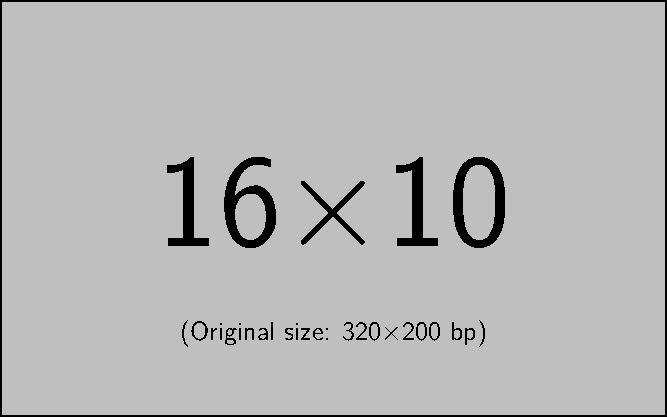
\includegraphics[width=0.75\linewidth]{example-image-16x10.pdf}
\caption{Insert figure caption here}
\label{fig_sim}
\end{figure}


\begin{figure*}
\centering
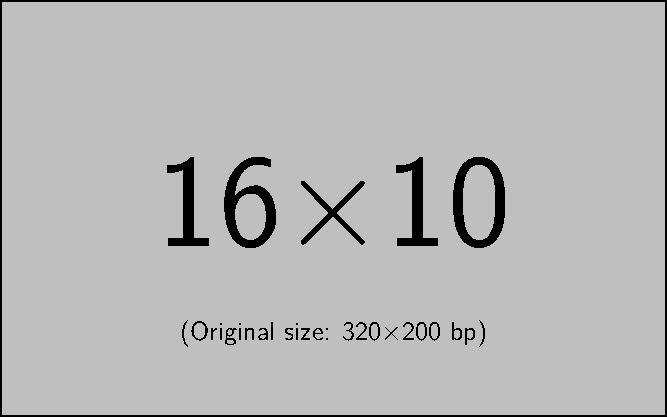
\includegraphics[width=0.8\linewidth]{example-image-16x10.pdf}
\caption{Insert figure caption here}
\label{fig_wide}
\end{figure*}


See example table in Table~\ref{table_example}.

\begin{table}[hbt!]
\begin{threeparttable}
\caption{An Example of a Table}
\label{table_example}
\begin{tabular}{llll}
\toprule
\headrow Column head 1 & Column head 2  & Column head 3 & Column head 4\\
\midrule
One\tnote{a} & Two&three three &four\\ 
\midrule
Three & Four&three three\tnote{b} &four\\
\bottomrule
\end{tabular}
\begin{tablenotes}[hang]
\item[]Table note
\item[a]First note
\item[b]Another table note
\end{tablenotes}
\end{threeparttable}
\end{table}


\section{Conclusion}
The conclusion text goes here.


\begin{acknowledgement}
Insert the Acknowledgment text here.
\end{acknowledgement}

\paragraph{Funding Statement}

This research was supported by grants from the <funder-name> <doi> (<award ID>); <funder-name> <doi> (<award ID>).

\paragraph{Competing Interests}

A statement about any financial, professional, contractual or personal relationships or situations that could be perceived to impact the presentation of the work --- or `None' if none exist.

\paragraph{Data Availability Statement}

A statement about how to access data, code and other materials allowing users to understand, verify and replicate findings --- e.g. Replication data and code can be found in Harvard Dataverse: \verb+\url{https://doi.org/link}+.



%\endnote in some journals will behave like \footnote; and \printendnotes will not output anything. 
\printendnotes

% \printbibliography

\appendix

\section{Example Appendix Section}

Lorem ipsum dolor sit amet, consectetur adipiscing elit, sed do eiusmod tempor incididunt ut labore et dolore magna aliqua. Lorem ipsum dolor sit amet, consectetur adipiscing elit, sed do eiusmod tempor incididunt ut labore et dolore magna aliqua. Lorem ipsum dolor sit amet, consectetur adipiscing elit, sed do eiusmod tempor incididunt ut labore et dolore magna aliqua. 


\end{document}
